\documentclass{article} % For LaTeX2e
\usepackage{nips14submit_e,times}
\usepackage{hyperref}
\usepackage{url}
\usepackage{graphicx}
\graphicspath{ {fig/} }
\usepackage{amsmath}
\usepackage{subfigure}
%\documentstyle[nips14submit_09,times,art10]{article} % For LaTeX 2.09


\title{EM Algorithm with Genetic Evolution}


\author{
David S.~Hippocampus\thanks{ Use footnote for providing further information
about author (webpage, alternative address)---\emph{not} for acknowledging
funding agencies.} \\
Department of Computer Science\\
Cranberry-Lemon University\\
Pittsburgh, PA 15213 \\
\texttt{hippo@cs.cranberry-lemon.edu} \\
\And
Coauthor \\
Affiliation \\
Address \\
\texttt{email} \\
\AND
Coauthor \\
Affiliation \\
Address \\
\texttt{email} \\
\And
Coauthor \\
Affiliation \\
Address \\
\texttt{email} \\
\And
Coauthor \\
Affiliation \\
Address \\
\texttt{email} \\
(if needed)\\
}

% The \author macro works with any number of authors. There are two commands
% used to separate the names and addresses of multiple authors: \And and \AND.
%
% Using \And between authors leaves it to \LaTeX{} to determine where to break
% the lines. Using \AND forces a linebreak at that point. So, if \LaTeX{}
% puts 3 of 4 authors names on the first line, and the last on the second
% line, try using \AND instead of \And before the third author name.

\newcommand{\fix}{\marginpar{FIX}}
\newcommand{\new}{\marginpar{NEW}}

\nipsfinalcopy % Uncomment for camera-ready version

\begin{document}


\maketitle

\begin{abstract}
The abstract paragraph should be indented 1/2~inch (3~picas) on both left and
right-hand margins. Use 10~point type, with a vertical spacing of 11~points.
The word \textbf{Abstract} must be centered, bold, and in point size 12. Two
line spaces precede the abstract. The abstract must be limited to one
paragraph.
\end{abstract}

%%%%%%%%%%%%%%%%%%%%%%%%%%%%%%%%%%%%%%%%%%%%%%%%%%%%%%%%%%%%%%%%%%%%%%%%%%%%%
\section{Introduction}
%%%%%%%%%%%%%%%%%%%%%%%%%%%%%%%%%%%%%%%%%%%%%%%%%%%%%%%%%%%%%%%%%%%%%%%%%%%%%

\subsection{Motivation}

\subsection{Genetic algorithm}


%%%%%%%%%%%%%%%%%%%%%%%%%%%%%%%%%%%%%%%%%%%%%%%%%%%%%%%%%%%%%%%%%%%%%%%%%%%%%
\section{Method: genetic-based EM algorithm (GA-EM)}
%%%%%%%%%%%%%%%%%%%%%%%%%%%%%%%%%%%%%%%%%%%%%%%%%%%%%%%%%%%%%%%%%%%%%%%%%%%%%

\subsection{Model selection criterion: MDL}

\subsection{Encoding}

Each individual in the population is composed of three parts, as shown in Figure~\ref{fig:encoding}. The first part (Part A) uses binary encoding, where the total number of bits is determined by the maximal number of allowed components $M_{\max}$. Each bit represents one particular Gaussian component in the model. If the bit is set to 0, then its associated component is omitted for modeling the mixture. In contrast, if the bit is set to 1, then it means this component is responsible for some data points in the mixture. The second part (Part B) uses floating point value encoding to record the components weight $\mathbf{w}$ of which the length is $M_{\max}$. Note that due to the switching mechanism of the components among individuals during evolution, the weight might need to be reset to uniform distribution except for the best individual (elitist). And the principle is to keep the weight as long as possible. The third part (Part C) also uses floating point value encoding to record the mean $\boldsymbol{\mu_m}$ and covariance $\boldsymbol{\Sigma_m}$ (and maybe other parameters) of the $M_{\max}$ components. 


\begin{figure}[h]
\begin{center}
\includegraphics[scale=0.3]{encoding.jpg}
\end{center}
\caption{Encoding of individuals.}
\label{fig:encoding}
\end{figure}

 
\subsection{Recombination}

The crossover operator selects two parent individuals randomly from the current population $\mathbf{P}$ and recombines them to form two offsprings. Total number of $H$ ($H<K$ and is a multiple of 2) children will be generated in this step. We use \textit{single-point crossover} (\textbf{TOCITE}), which chooses randomly a cross-over position $\chi = \{1, \ldots, M_{\max}\}$ within Part A of the individual and exchanges the value of the genes to the right of this position between two selected parent individuals, as shown in Figure~\ref{fig:recombination}. Part B of the offsprings are set to uniform distribution and Part C are exchanged correspondingly.

\begin{figure}[h]
\begin{center}
\includegraphics[scale=0.3]{recombination.jpg}
\end{center}
\caption{Recombination: single-point crossover.}
\label{fig:recombination}
\end{figure}

\subsection{Selection}

\subsection{Enforced mutation}

\subsection{Mutation}

\subsection{Implementation}



%%%%%%%%%%%%%%%%%%%%%%%%%%%%%%%%%%%%%%%%%%%%%%%%%%%%%%%%%%%%%%%%%%%%%%%%%%%%%
\section{Results and Discussion}
%%%%%%%%%%%%%%%%%%%%%%%%%%%%%%%%%%%%%%%%%%%%%%%%%%%%%%%%%%%%%%%%%%%%%%%%%%%%%

\subsection{Initialization}

The start population $\mathbf{P^0}$ is composed of a set of $K$ individuals, where each individual has randomly selected $M$ components. We explored two initialization methods:
\begin{enumerate}
\item \textit{random}: The mean values of each component $\boldsymbol{\mu^0_m}$ are set to randomly selected data points. The covariance matrices $\boldsymbol{\Sigma^0_m}$ are initialized as the sample covariance matrix of all data. The weights $\mathbf{w^0_m}$ of the components are assumed to be uniformly distributed.
\item \textit{k-means}: The parameters of the selected components are initialized by the k-means algorithm with $k=M$. The mean values of each component $\boldsymbol{\mu^0_m}$ are set to the cluster centroids. The covariance matrices $\boldsymbol{\Sigma^0_m}$ are initialized to the sample covariance matrices of the data in the corresponding cluster. The weights $\mathbf{w^0_m}$ of the components are the responsibilities of each cluster.
\end{enumerate}

\begin{figure}[htp]
  \begin{center}
    \subfigure[]{\includegraphics[width=6.8cm]{init_syn_1.pdf}}
    \subfigure[]{\includegraphics[width=6.8cm]{init_penpca_1.pdf}}
  \end{center}
  \caption{Various edge detection algorithms}
  \label{fig:edge}
\end{figure}

\subsection{Model selection}

\begin{figure}[h]
\begin{center}
\makebox[\textwidth][c]{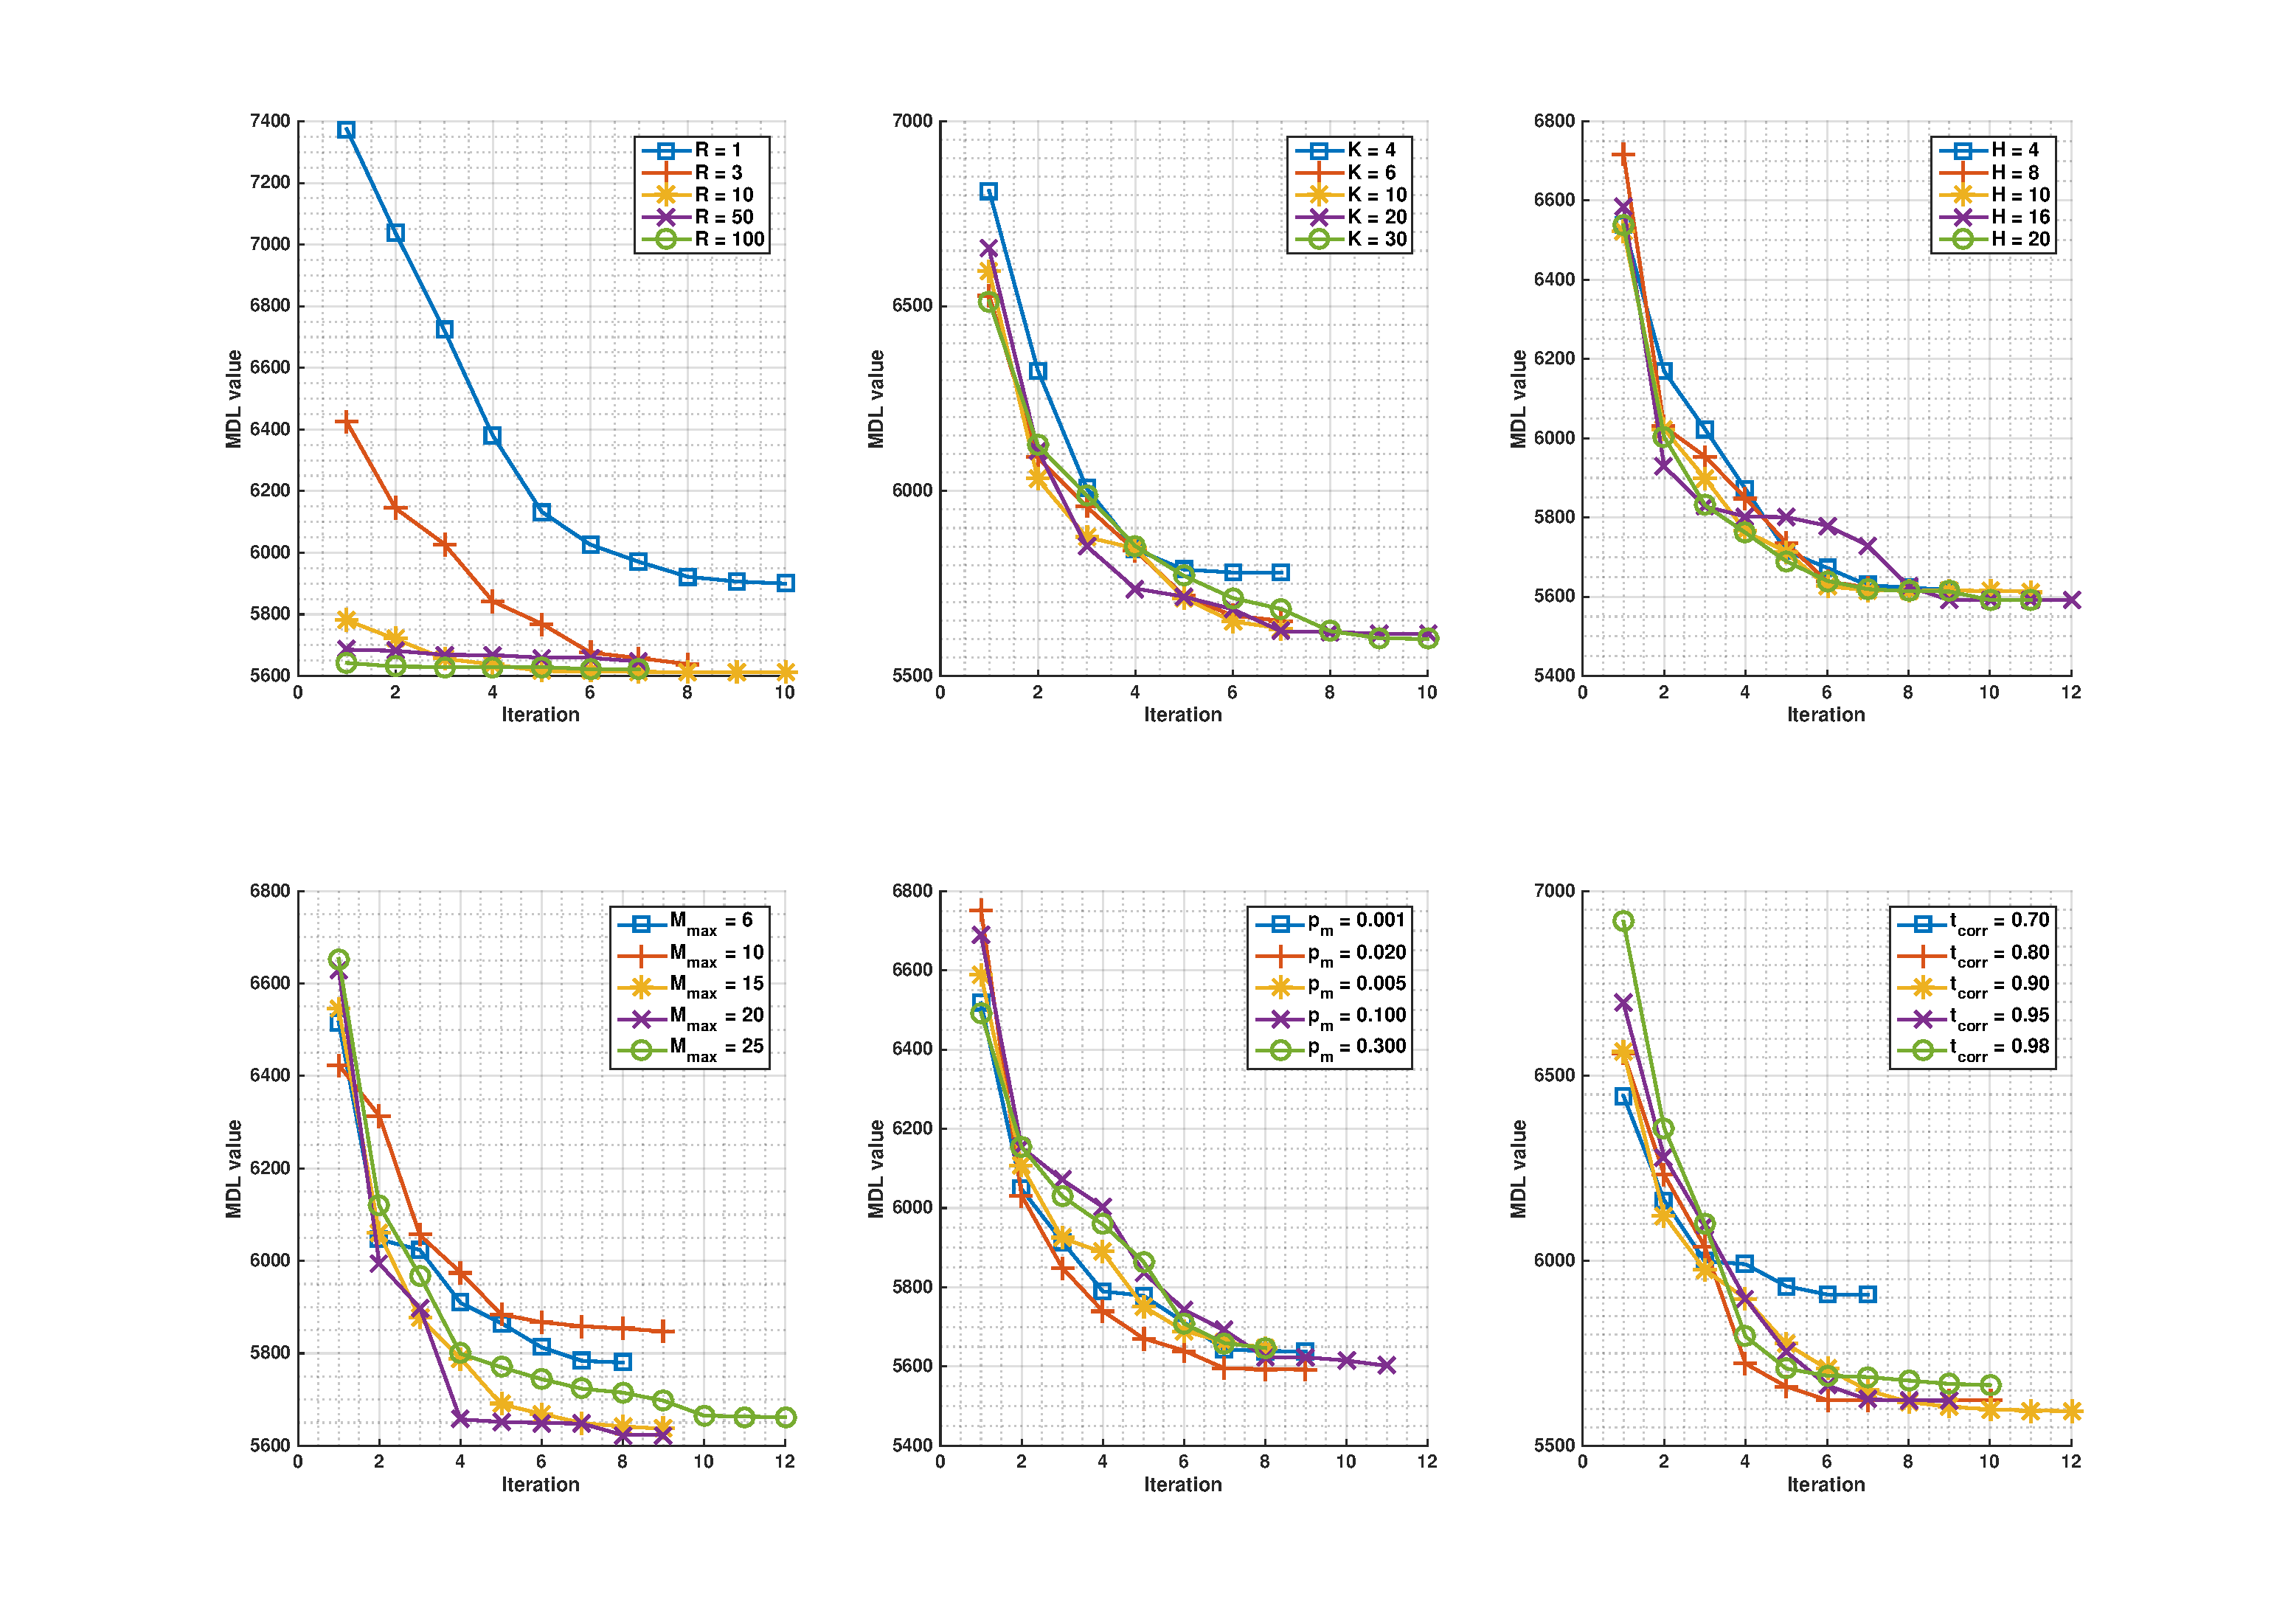
\includegraphics[scale=0.4]{model_sel_syn_1.pdf}}
\end{center}
\caption{Encoding of individuals.}
\label{fig:mod_sel_syn}
\end{figure}

\begin{figure}[h]
\begin{center}
\makebox[\textwidth][c]{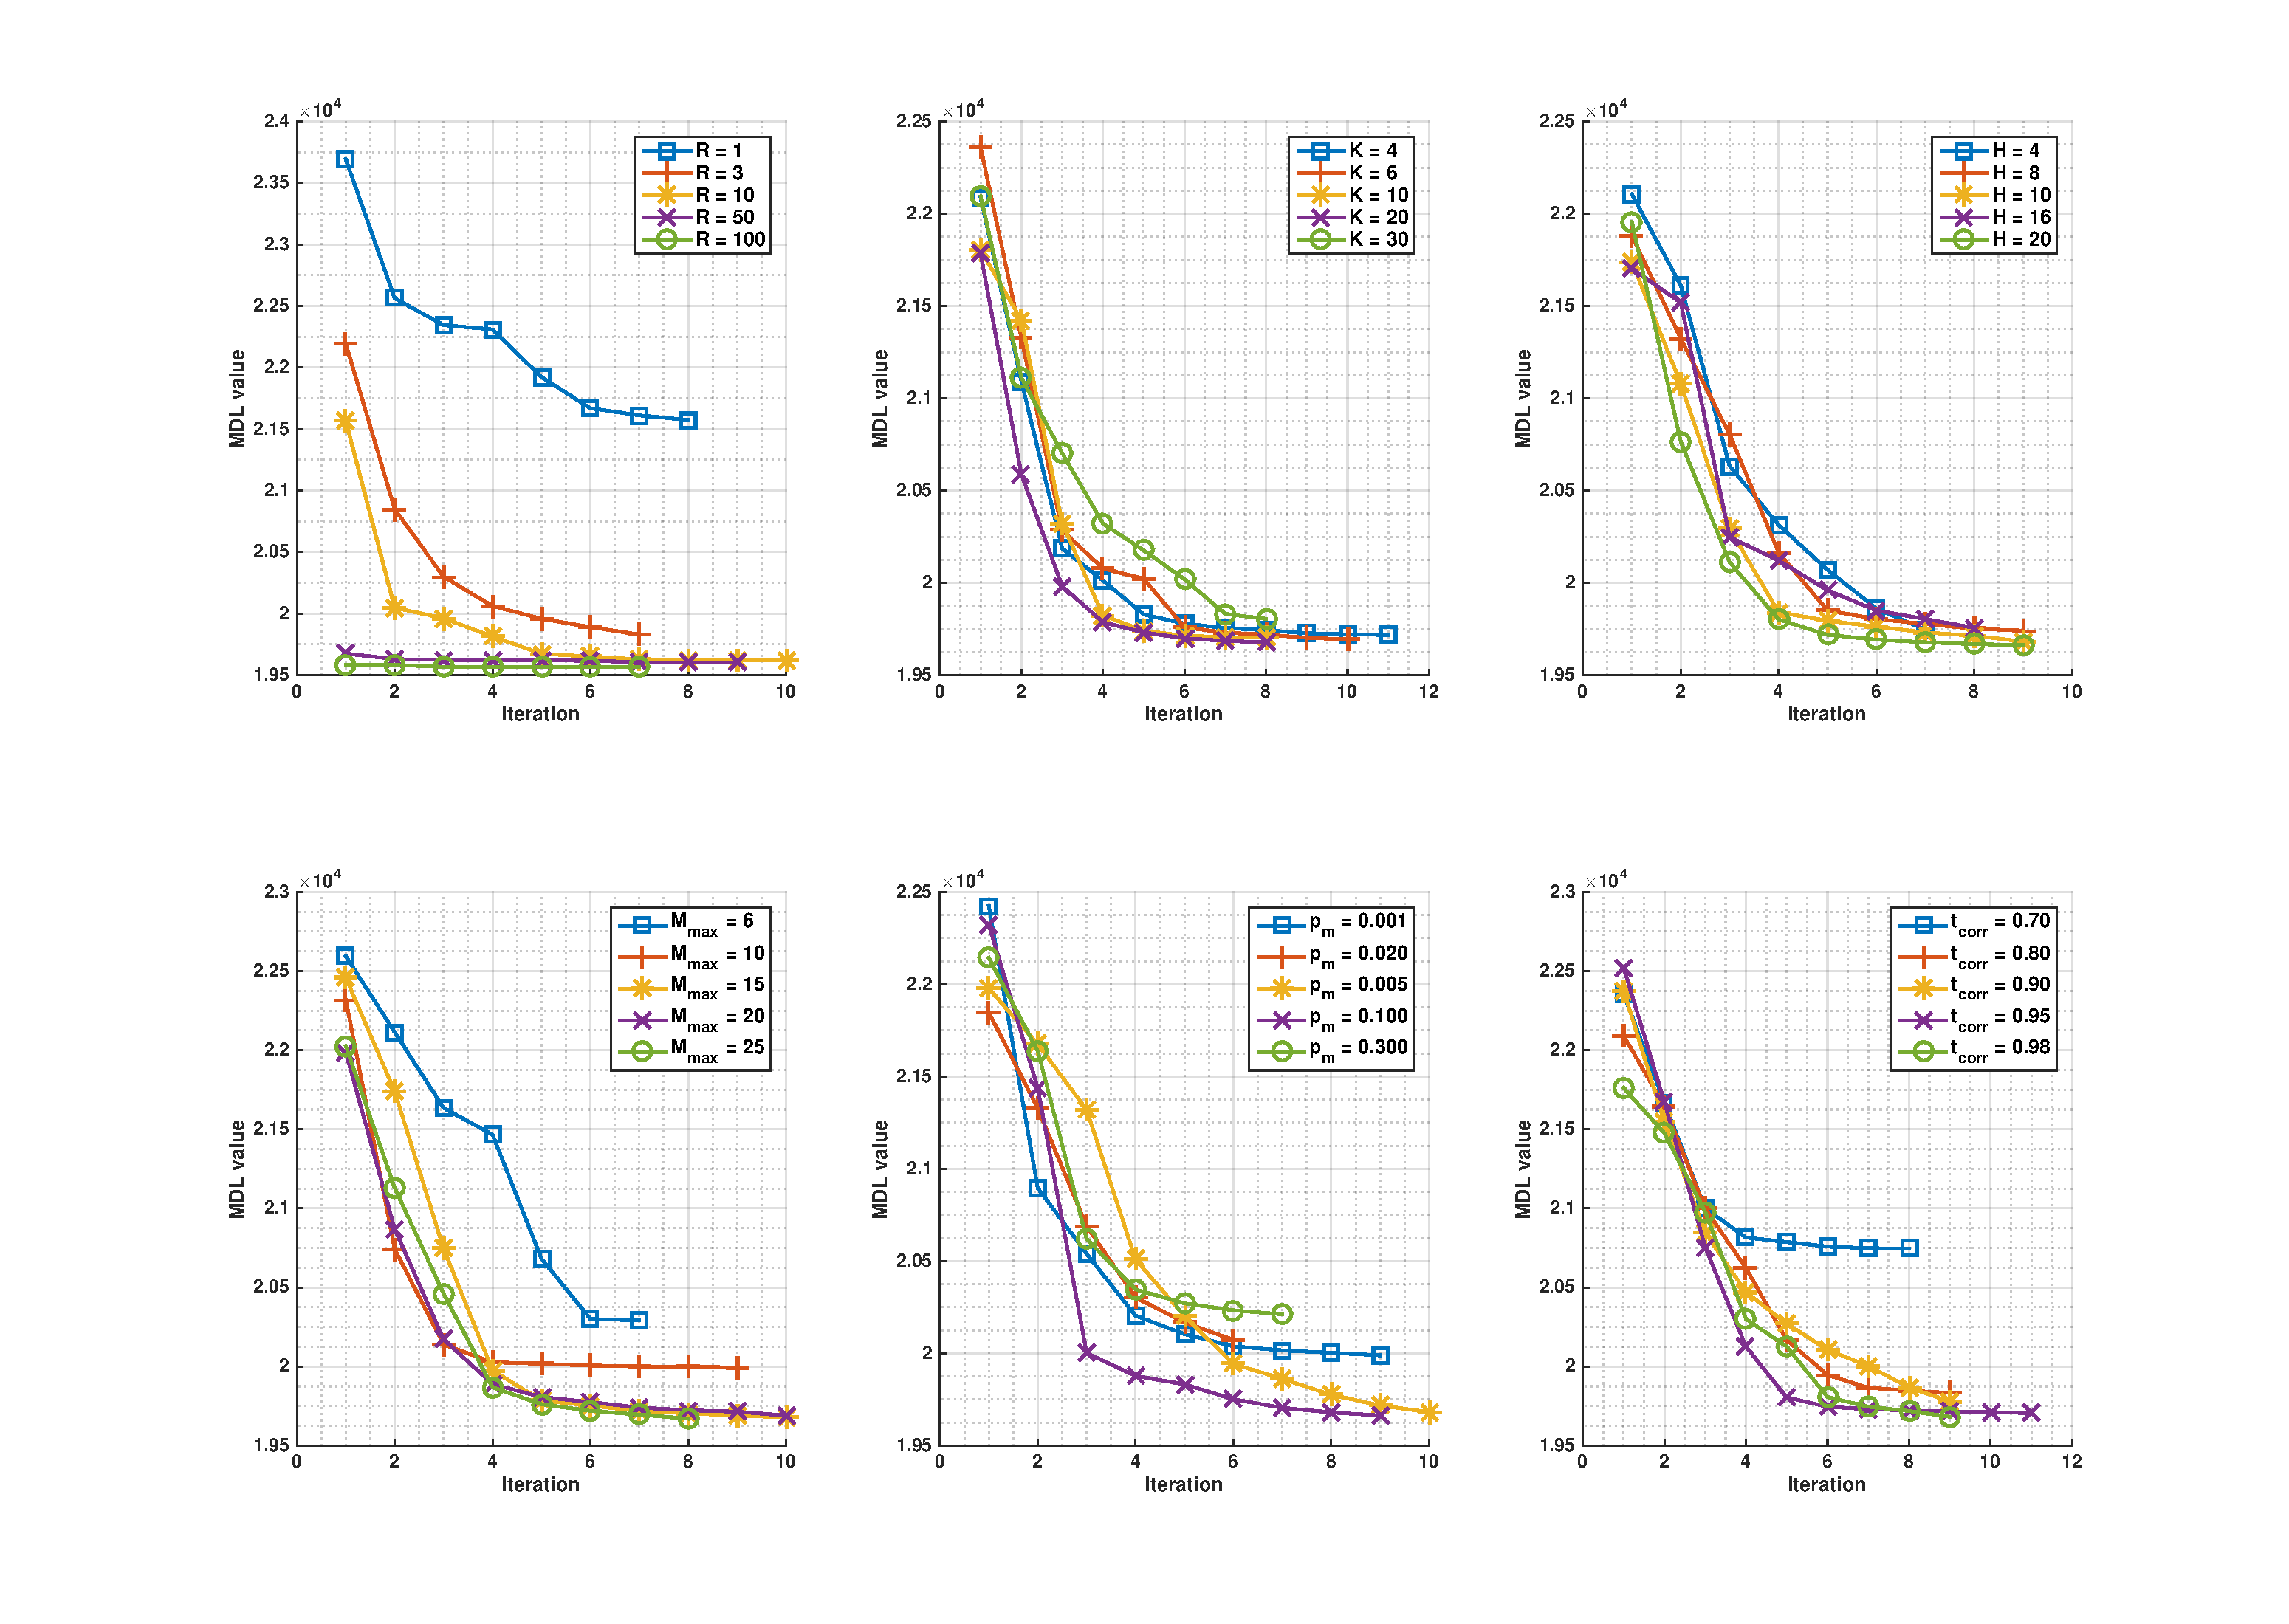
\includegraphics[scale=0.4]{model_sel_penpca_1.pdf}}
\end{center}
\caption{Encoding of individuals.}
\label{fig:mod_sel_penpca}
\end{figure}
 
\subsection{Application on real data}

\subsection{Performance}

\subsection{Extension of GA-EM}


%%%%%%%%%%%%%%%%%%%%%%%%%%%%%%%%%%%%%%%%%%%%%%%%%%%%%%%%%%%%%%%%%%%%%%%%%%%%%
\section{Summary and future work}
%%%%%%%%%%%%%%%%%%%%%%%%%%%%%%%%%%%%%%%%%%%%%%%%%%%%%%%%%%%%%%%%%%%%%%%%%%%%%



\section{General formatting instructions}
\label{gen_inst}

The text must be confined within a rectangle 5.5~inches (33~picas) wide and
9~inches (54~picas) long. The left margin is 1.5~inch (9~picas).
Use 10~point type with a vertical spacing of 11~points. Times New Roman is the
preferred typeface throughout. Paragraphs are separated by 1/2~line space,
with no indentation.

Paper title is 17~point, initial caps/lower case, bold, centered between
2~horizontal rules. Top rule is 4~points thick and bottom rule is 1~point
thick. Allow 1/4~inch space above and below title to rules. All pages should
start at 1~inch (6~picas) from the top of the page.

%The version of the paper submitted for review should have ``Anonymous Author(s)'' as the author of the paper.

For the final version, authors' names are
set in boldface, and each name is centered above the corresponding
address. The lead author's name is to be listed first (left-most), and
the co-authors' names (if different address) are set to follow. If
there is only one co-author, list both author and co-author side by side.

Please pay special attention to the instructions in section \ref{others}
regarding figures, tables, acknowledgments, and references.

\section{Headings: first level}
\label{headings}

First level headings are lower case (except for first word and proper nouns),
flush left, bold and in point size 12. One line space before the first level
heading and 1/2~line space after the first level heading.

\subsection{Headings: second level}

Second level headings are lower case (except for first word and proper nouns),
flush left, bold and in point size 10. One line space before the second level
heading and 1/2~line space after the second level heading.

\subsubsection{Headings: third level}

Third level headings are lower case (except for first word and proper nouns),
flush left, bold and in point size 10. One line space before the third level
heading and 1/2~line space after the third level heading.

\section{Citations, figures, tables, references}
\label{others}

These instructions apply to everyone, regardless of the formatter being used.

\subsection{Citations within the text}

Citations within the text should be numbered consecutively. The corresponding
number is to appear enclosed in square brackets, such as [1] or [2]-[5]. The
corresponding references are to be listed in the same order at the end of the
paper, in the \textbf{References} section. (Note: the standard
\textsc{Bib\TeX} style \texttt{unsrt} produces this.) As to the format of the
references themselves, any style is acceptable as long as it is used
consistently.

As submission is double blind, refer to your own published work in the 
third person. That is, use ``In the previous work of Jones et al.\ [4]'',
not ``In our previous work [4]''. If you cite your other papers that
are not widely available (e.g.\ a journal paper under review), use
anonymous author names in the citation, e.g.\ an author of the
form ``A.\ Anonymous''. 


\subsection{Footnotes}

Indicate footnotes with a number\footnote{Sample of the first footnote} in the
text. Place the footnotes at the bottom of the page on which they appear.
Precede the footnote with a horizontal rule of 2~inches
(12~picas).\footnote{Sample of the second footnote}

\subsection{Figures}

All artwork must be neat, clean, and legible. Lines should be dark
enough for purposes of reproduction; art work should not be
hand-drawn. The figure number and caption always appear after the
figure. Place one line space before the figure caption, and one line
space after the figure. The figure caption is lower case (except for
first word and proper nouns); figures are numbered consecutively.

Make sure the figure caption does not get separated from the figure.
Leave sufficient space to avoid splitting the figure and figure caption.

You may use color figures. 
However, it is best for the
figure captions and the paper body to make sense if the paper is printed
either in black/white or in color.
\begin{figure}[h]
\begin{center}
%\framebox[4.0in]{$\;$}
\fbox{\rule[-.5cm]{0cm}{4cm} \rule[-.5cm]{4cm}{0cm}}
\end{center}
\caption{Sample figure caption.}
\end{figure}

\subsection{Tables}

All tables must be centered, neat, clean and legible. Do not use hand-drawn
tables. The table number and title always appear before the table. See
Table~\ref{sample-table}.

Place one line space before the table title, one line space after the table
title, and one line space after the table. The table title must be lower case
(except for first word and proper nouns); tables are numbered consecutively.

\begin{table}[t]
\caption{Sample table title}
\label{sample-table}
\begin{center}
\begin{tabular}{ll}
\multicolumn{1}{c}{\bf PART}  &\multicolumn{1}{c}{\bf DESCRIPTION}
\\ \hline \\
Dendrite         &Input terminal \\
Axon             &Output terminal \\
Soma             &Cell body (contains cell nucleus) \\
\end{tabular}
\end{center}
\end{table}

\section{Final instructions}
Do not change any aspects of the formatting parameters in the style files.
In particular, do not modify the width or length of the rectangle the text
should fit into, and do not change font sizes (except perhaps in the
\textbf{References} section; see below). Please note that pages should be
numbered.

\section{Preparing PostScript or PDF files}

Please prepare PostScript or PDF files with paper size ``US Letter'', and
not, for example, ``A4''. The -t
letter option on dvips will produce US Letter files.

Fonts were the main cause of problems in the past years. Your PDF file must
only contain Type 1 or Embedded TrueType fonts. Here are a few instructions
to achieve this.

\begin{itemize}

\item You can check which fonts a PDF files uses.  In Acrobat Reader,
select the menu Files$>$Document Properties$>$Fonts and select Show All Fonts. You can
also use the program \verb+pdffonts+ which comes with \verb+xpdf+ and is
available out-of-the-box on most Linux machines.

\item The IEEE has recommendations for generating PDF files whose fonts
are also acceptable for NIPS. Please see
\url{http://www.emfield.org/icuwb2010/downloads/IEEE-PDF-SpecV32.pdf}

\item LaTeX users:

\begin{itemize}

\item Consider directly generating PDF files using \verb+pdflatex+
(especially if you are a MiKTeX user). 
PDF figures must be substituted for EPS figures, however.

\item Otherwise, please generate your PostScript and PDF files with the following commands:
\begin{verbatim} 
dvips mypaper.dvi -t letter -Ppdf -G0 -o mypaper.ps
ps2pdf mypaper.ps mypaper.pdf
\end{verbatim}

Check that the PDF files only contains Type 1 fonts. 
%For the final version, please send us both the Postscript file and
%the PDF file. 

\item xfig "patterned" shapes are implemented with 
bitmap fonts.  Use "solid" shapes instead. 
\item The \verb+\bbold+ package almost always uses bitmap
fonts.  You can try the equivalent AMS Fonts with command
\begin{verbatim}
\usepackage[psamsfonts]{amssymb}
\end{verbatim}
 or use the following workaround for reals, natural and complex: 
\begin{verbatim}
\newcommand{\RR}{I\!\!R} %real numbers
\newcommand{\Nat}{I\!\!N} %natural numbers 
\newcommand{\CC}{I\!\!\!\!C} %complex numbers
\end{verbatim}

\item Sometimes the problematic fonts are used in figures
included in LaTeX files. The ghostscript program \verb+eps2eps+ is the simplest
way to clean such figures. For black and white figures, slightly better
results can be achieved with program \verb+potrace+.
\end{itemize}
\item MSWord and Windows users (via PDF file):
\begin{itemize}
\item Install the Microsoft Save as PDF Office 2007 Add-in from
\url{http://www.microsoft.com/downloads/details.aspx?displaylang=en\&familyid=4d951911-3e7e-4ae6-b059-a2e79ed87041}
\item Select ``Save or Publish to PDF'' from the Office or File menu
\end{itemize}
\item MSWord and Mac OS X users (via PDF file):
\begin{itemize}
\item From the print menu, click the PDF drop-down box, and select ``Save
as PDF...''
\end{itemize}
\item MSWord and Windows users (via PS file):
\begin{itemize}
\item To create a new printer
on your computer, install the AdobePS printer driver and the Adobe Distiller PPD file from
\url{http://www.adobe.com/support/downloads/detail.jsp?ftpID=204} {\it Note:} You must reboot your PC after installing the
AdobePS driver for it to take effect.
\item To produce the ps file, select ``Print'' from the MS app, choose
the installed AdobePS printer, click on ``Properties'', click on ``Advanced.''
\item Set ``TrueType Font'' to be ``Download as Softfont''
\item Open the ``PostScript Options'' folder
\item Select ``PostScript Output Option'' to be ``Optimize for Portability''
\item Select ``TrueType Font Download Option'' to be ``Outline''
\item Select ``Send PostScript Error Handler'' to be ``No''
\item Click ``OK'' three times, print your file.
\item Now, use Adobe Acrobat Distiller or ps2pdf to create a PDF file from
the PS file. In Acrobat, check the option ``Embed all fonts'' if
applicable.
\end{itemize}

\end{itemize}
If your file contains Type 3 fonts or non embedded TrueType fonts, we will
ask you to fix it. 

\subsection{Margins in LaTeX}
 
Most of the margin problems come from figures positioned by hand using
\verb+\special+ or other commands. We suggest using the command
\verb+\includegraphics+
from the graphicx package. Always specify the figure width as a multiple of
the line width as in the example below using .eps graphics
\begin{verbatim}
   \usepackage[dvips]{graphicx} ... 
   \includegraphics[width=0.8\linewidth]{myfile.eps} 
\end{verbatim}
or % Apr 2009 addition
\begin{verbatim}
   \usepackage[pdftex]{graphicx} ... 
   \includegraphics[width=0.8\linewidth]{myfile.pdf} 
\end{verbatim}
for .pdf graphics. 
See section 4.4 in the graphics bundle documentation (\url{http://www.ctan.org/tex-archive/macros/latex/required/graphics/grfguide.ps}) 
 
A number of width problems arise when LaTeX cannot properly hyphenate a
line. Please give LaTeX hyphenation hints using the \verb+\-+ command.


\subsubsection*{Acknowledgments}

Use unnumbered third level headings for the acknowledgments. All
acknowledgments go at the end of the paper. Do not include 
acknowledgments in the anonymized submission, only in the 
final paper. 

\subsubsection*{References}

References follow the acknowledgments. Use unnumbered third level heading for
the references. Any choice of citation style is acceptable as long as you are
consistent. It is permissible to reduce the font size to `small' (9-point) 
when listing the references. {\bf Remember that this year you can use
a ninth page as long as it contains \emph{only} cited references.}

\small{
[1] Alexander, J.A. \& Mozer, M.C. (1995) Template-based algorithms
for connectionist rule extraction. In G. Tesauro, D. S. Touretzky
and T.K. Leen (eds.), {\it Advances in Neural Information Processing
Systems 7}, pp. 609-616. Cambridge, MA: MIT Press.

[2] Bower, J.M. \& Beeman, D. (1995) {\it The Book of GENESIS: Exploring
Realistic Neural Models with the GEneral NEural SImulation System.}
New York: TELOS/Springer-Verlag.

[3] Hasselmo, M.E., Schnell, E. \& Barkai, E. (1995) Dynamics of learning
and recall at excitatory recurrent synapses and cholinergic modulation
in rat hippocampal region CA3. {\it Journal of Neuroscience}
{\bf 15}(7):5249-5262.
}

\end{document}
